"`Marktanalysen sind die Grundlage für wichtige strategische Geschäftsentscheidungen. 
Nicht nur Standortentscheidungen und die Wahl von Marketingmaßnahmen hängen davon ab, sie können – je nach 
Schwerpunkt – auch ausschlaggebende Informationen zur Preispolitik, Expansionsplänen und Produktentwicklung 
beisteuern. So helfen sie etwa dabei, dass ein Markteintritt oder die Neueinführung eines Produktes gelingt
oder ganz neue Märkte erschlossen werden können. "'
\cite{marktanalyse}

\section{Vorgehensweise}

In einem ersten Schritt wird der Markt und die Zielgruppe definiert. 
Ist die App global verfügbar oder nur in bestimmten Regionen? Wer sind die potenziellen Benutzer:innen?
Wie viel Interesse besteht an der App von den Kund:innen?

In einem nächsten Schritt muss der Wettbewerb untersucht werden.
Welche Entspannungsapps sind auf dem Markt, welche davon sind am erfolgreichsten und warum?
Dazu kommt noch eine Bewertung der aktuellen Trends im Bereich Gesundheit und Wohlbefinden. 
Gibt es aktuelle oder neue Technologien oder Forschungsergebnisse, die in die App integriert werden könnten?

Danach werden verschiedene Geschäftsmodelle in Erwägung gezogen. 
Soll die App kostenlos sein und durch Anzeigen oder In-App-Käufe finanziert werden? 
Oder wird es eine kostenpflichtige Premium-Version geben, mit der man mehr Funktionen innerhalb der App freischaltet?

Schließlich muss eine Marketingstrategie entwickelt werden, um die Entspannungsapp bekannt zu machen und
in Umlauf zu bringen. 
Welche Kanäle sind am besten dazu geeignet, die gewünschten Zielgruppen zu erreichen?


\begin{figure}[H]
    \centering
    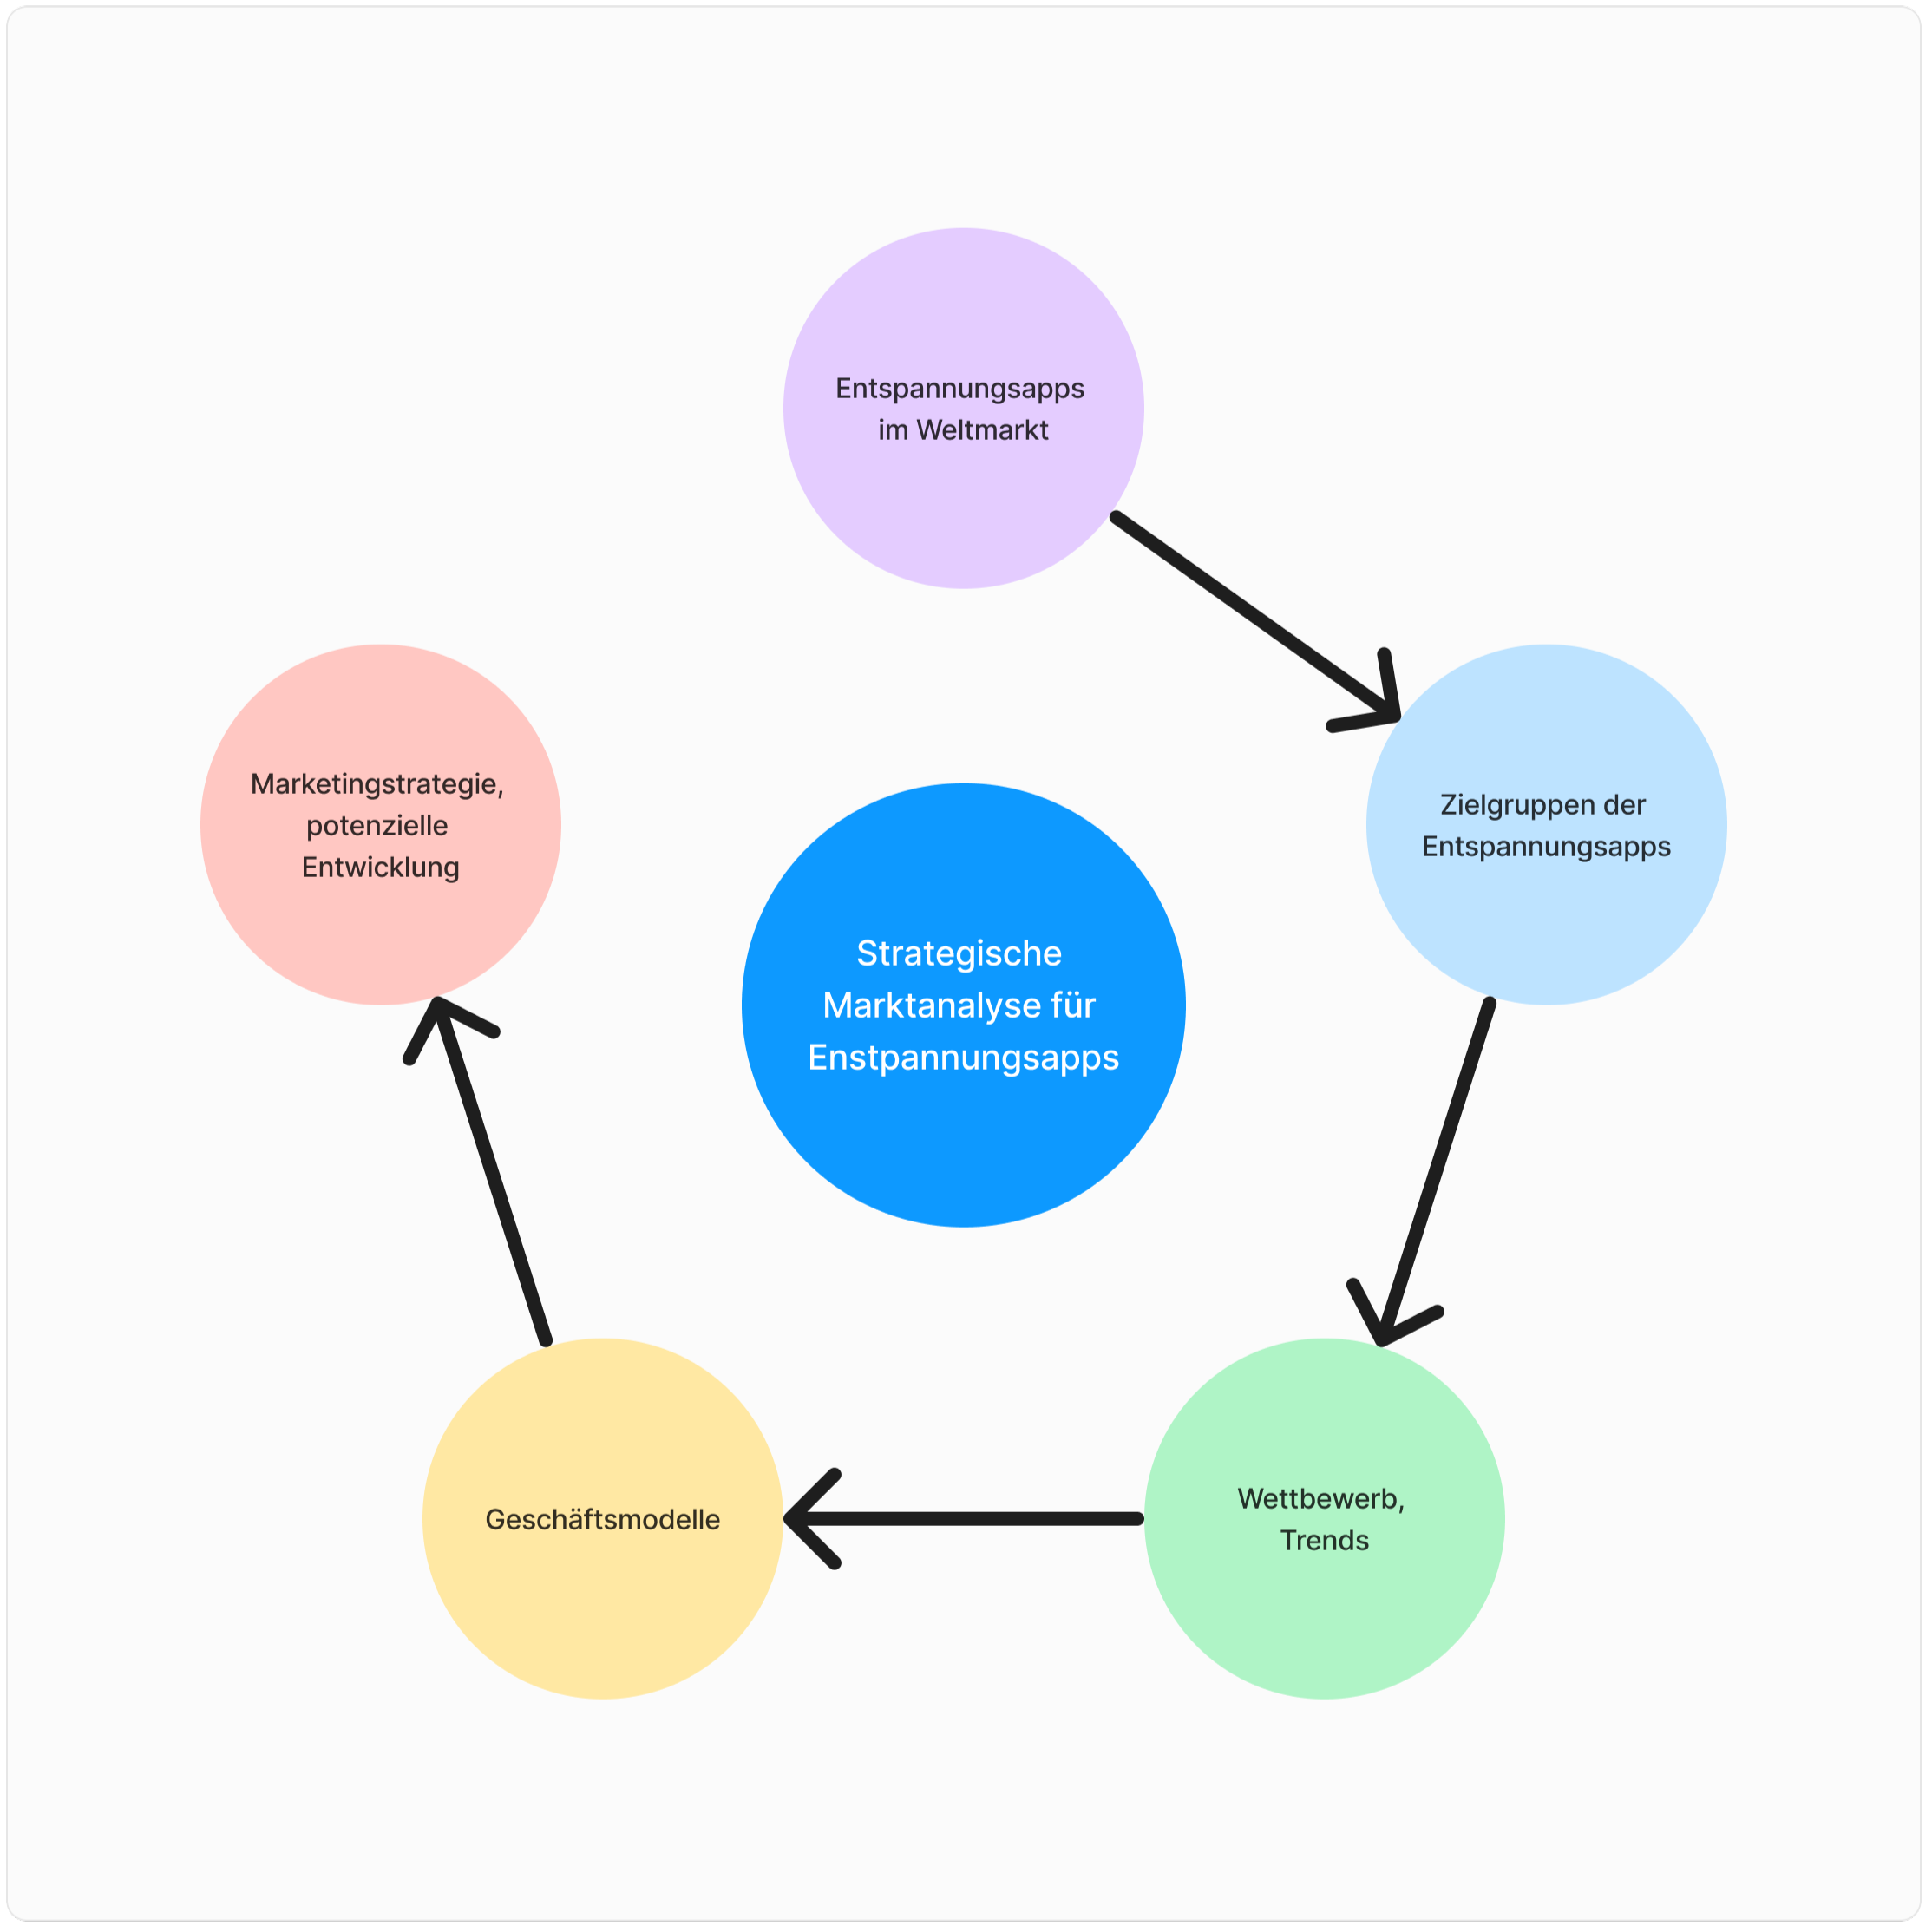
\includegraphics[height=\textwidth]{./pics/Marktanalyse-Relaxoon.png}
    \caption{Ablauf}
\end{figure}

Durch diese Analyse erhält man wichtige Erkenntnisse über die aktuelle Situation sowie potenzielle Entwicklungen
auf dem Markt für Entspannungsapps.


\section{Analyse}

Wie schon bei der Planung des Projektes formuliert wurde, soll die App Relaxoon, welche Stress bei bedürftigen 
Personen reduziert, im Play Store und im App Store 
international verfügbar sein. Der Markt bei Entspannungsapps
ist sehr groß, was zu hoher Konkurrenz führt. 

\subsection{Wettbewerb und Trends}

Einerseits gibt es viele Content-Creator, die ihre selbst erstellten Entspannungsmedien und -übungen, 
ohne die Verwendung einer konkreten 
Entspannungsapp, auf den bekanntesten und
auch größten Plattformen wie zum Beispiel YouTube oder Spotify direkt hochladen.
Das könnte bei einigen Menschen dazu führen, sich gar keine App installieren zu wollen, weil es unnötig erscheint.
Andererseits bieten Apps, die extra auf Entspannung konzipiert sind, massive Vorteile. 

Einige markante Features von Entspannungsapps sind:

\begin{itemize}
    \item Kurse, die eine Reihe von Entspannungsübungen in gezielter Reihenfolge bereitstellen
    \item Viele verschiedene Funktionen zum Abspielen von beruhigenden Geräuschen und Musik
    \item Anleitungen zur Meditation, welche ebenfalls als Einschlafhilfe dienen und für einen besseren Schlaf sorgen
\end{itemize}

Bei Entspannungsapps gibt es auch verschiedene Arten. Zum einen welche, die sich ausschließlich auf Meditation
spezialisiert haben, wohingegen andere nur audiovisuelle Inhalte zur Verfügung stellen. Es gibt ebenfalls Apps auf
dem Markt, die ausschließlich Spiele innerhalb der App zur Entspannung implementiert haben. 

Die Funktion von spielerischem Entspannen soll in Relaxoon nicht enthalten sein. Relaxoon soll
die Möglichkeit bieten, alle Bedürfnisse der User:innen abzudecken, wobei man sich persönlich als User:in 
auch dafür entscheiden kann, nach bestimmten Vorgaben zu filtern.

\begin{figure}[H]
    \centering
    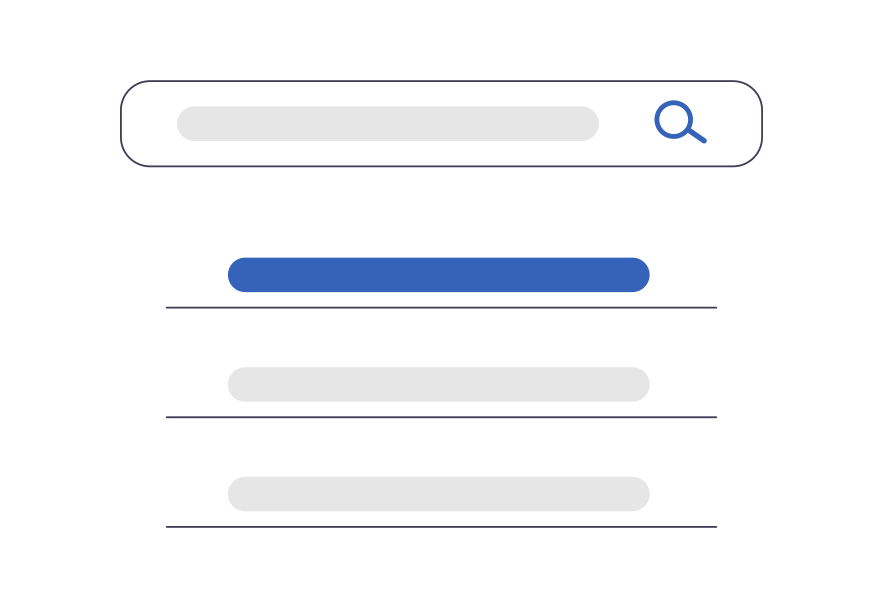
\includegraphics[height=0.35\textwidth]{./pics/undraw_Search_re_x5gq.png}
    \caption{}
\end{figure}

Man kann sich also dafür entscheiden, einen Text
zum Entspannen zu lesen, ruhige Musik zu hören, sich ein entspannendes Video anzusehen, oder eine eigene Übung
zu machen, in der mehrere Sinne angesprochen werden.

\subsection{Geschäftsmodelle}

Bei den Geschäftsmodellen gibt es, wie bereits oben erwähnt, für eine Entspannungsapp verschiedene Varianten. 

\subsubsection{Werbung}

Das Prinzip von Werbung in der App wäre die erste Möglichkeit mit dem Projekt Geld zu verdienen. 
Es würde jedoch den Zweck, dass man sich bei der Verwendung der App entspannen soll, sehr stark negativ beeinflussen.
Wenn man sich zum Beispiel vor jeder Übung ein 30-sekündiges Werbevideo anschauen muss, oder wenn Pop-Up-Fenster 
auftauchen würden, die der Nutzer oder die Nutzerin ständig wegtippen müssten, um fortfahren zu können, wäre das
kontraproduktiv. Das würde
sehr viele Leute abschrecken und darin resultieren, dass die App häufig direkt wieder deinstalliert wird.

\subsubsection{Einzelne In-App-Käufe}

Das Prinzip von In-App-Käufen ist sehr viel ansprechender. Es behindert die Nutzer:innen in keiner Weise daran,
die App ohne Unterbrechungen zu verwenden. Man könnte In-App-Käufe den Kund:innen so anbieten, dass sie zum
Beispiel für eine kleine Summe eine Übung freischalten können, oder auch für eine höhere Summe gleich zehn komplette
Übungen auf einmal erwerben können. 

\subsubsection{Premium Version}

Die wahrscheinlich geeignetste Lösung für Monetarisierung ist eine Premium Version für Relaxoon zu verkaufen, mit
der man die gesamten Features der App benutzen kann. Diese könnte man einmalig bezahlbar machen, sodass die User:innen
für immer Zugriff auf Premium Inhalte bekommen, oder auch 
monatlich verrechnen, dass jeden Monat wie bei einem Abonnement gezahlt werden muss.

\newpage

Es wichtig zu erwähnen, dass man die App auch schon im Play- und im App Store käuflich machen könnte. Das würde
jedoch die Verbreitung und Reichweite der App einschränken, weil sich durch den Preis, der schon vorab zu bezahlen
wäre, weniger Leute die App tatsächlich kaufen und dann erst herunterladen würden. Eine von Grund auf kostenlose
App passt deswegen besser.

\subsubsection{Marketingstrategie}

Im Online- und Web-Marketing steht die Steigerung der Sichtbarkeit und die Umwandlung von Besuchern in zahlende 
Kunden im Vordergrund. Es wird oft auf Strategien wie Suchmaschinenoptimierung (SEO), Content-Marketing und 
Social-Media-Werbung gesetzt wird, um eine breite Online-Sichtbarkeit zu erreichen. Im Gegensatz dazu legt das 
App-Marketing den Fokus auf Aspekte wie App Store-Optimierung (ASO), gezielte 
Werbekampagnen innerhalb von App-Plattformen und die Schaffung einer positiven Nutzererfahrung, um sowohl die Anzahl 
der Downloads als auch das langfristige Engagement der Nutzer zu steigern.
\cite{marketingstrategie} 

Ein Problem, das häufig dabei entsteht ist, dass Personen eine App oft gar nicht lange installiert haben und oft diese 
schon nach nur einmaligem Nutzen wieder deinstallieren.

Auf der Website absatzwirtschaft.de wurde das noch genauer erläutert: \cite{deinstallieren}

\begin{quotation}
"`App-Marketer haben weniger als sechs Tage Zeit, um das Interesse von Nutzern erneut zu wecken: Der durchschnittliche
Nutzer wartet zwischen dem letzten Öffnen der App und der Deinstallation knapp sechs Tage. Dabei variiert die
Zeitspanne stark zwischen den einzelnen App-Kategorien – von weniger als drei Stunden bis zu etwa 15 Tagen.
Entertainment- und Lifestyle-Apps werden besonders schnell verworfen, ihre Nutzer deinstallieren Apps im Durchschnitt 
nach einem halben bis ganzen Tag. E-Commerce- und Reise-Apps hingegen haben eine wesentlich längere Lebensdauer und 
werden in der Regel zehn bis elf Tage nach der letzten Session eines Nutzers gelöscht."' 
\end{quotation}

\begin{figure}[H]
    \centering
    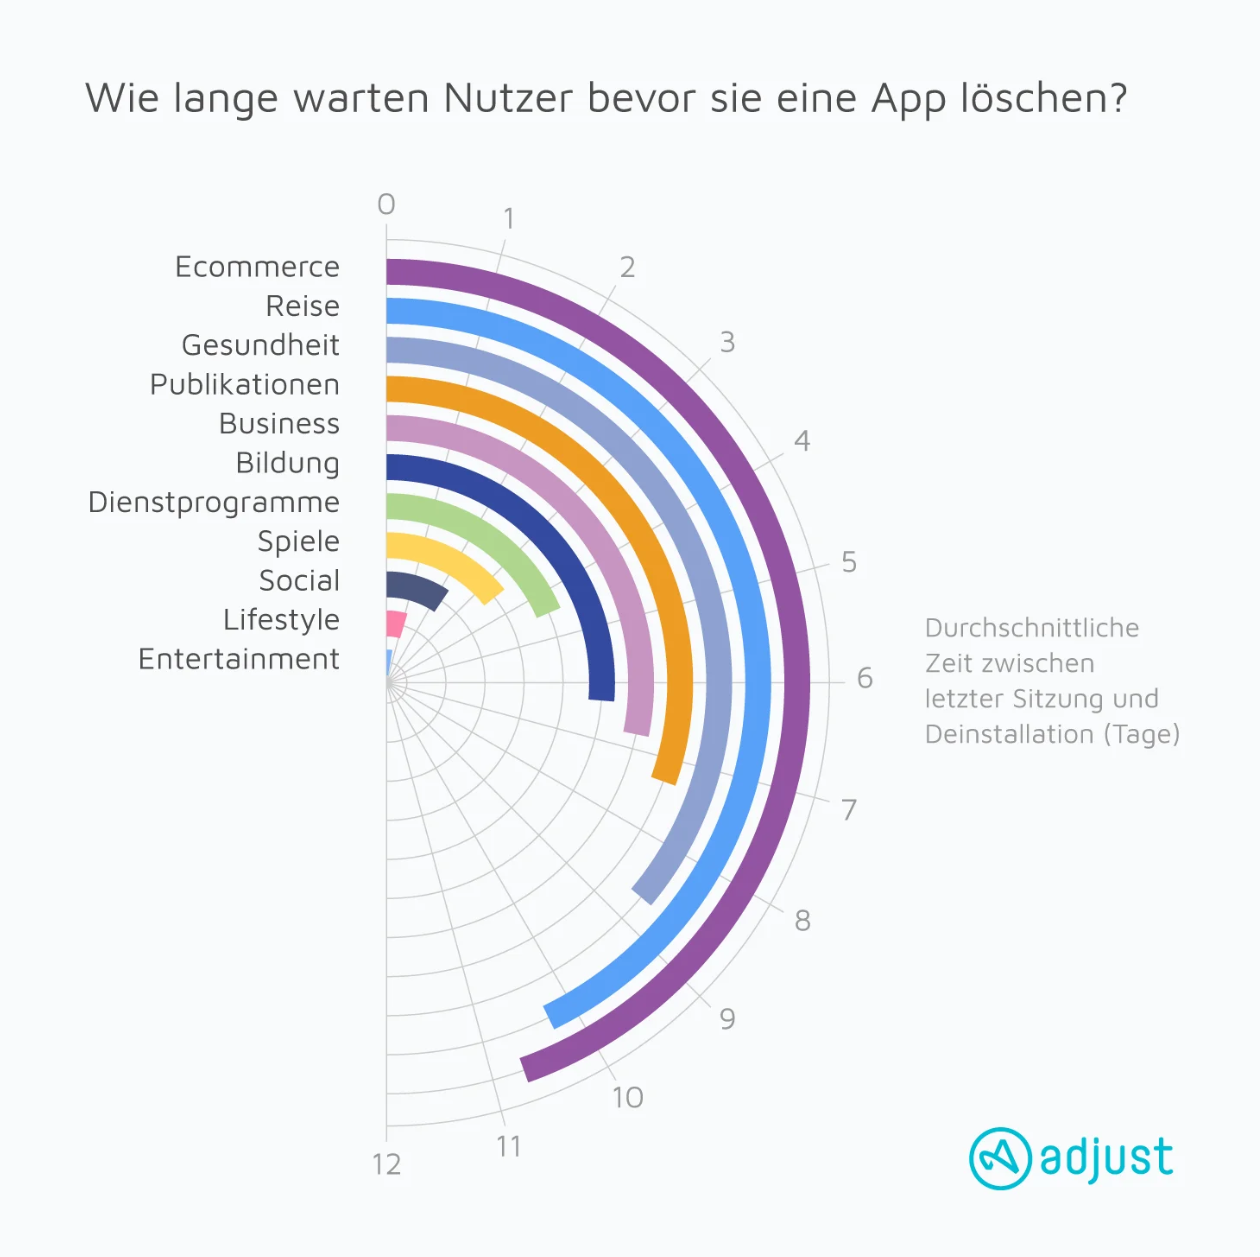
\includegraphics[height=\textwidth]{./pics/deinstallieren.png}
    \caption{App Statistik \cite{deinstallieren}}
\end{figure}
